\chapter{Parallelizing a Compiler}
\label{chap:proposta}

Having discussed both the theoretical and technical aspects of compilers, and
presented the previous works in the area, we discuss our attempts and success
of parallelizing a compiler.

%Como atestado por \cite{PR84402}, há um gargalo de paralelismo dentro do
%próprio GCC por conta de arquivos grandes. Outro gargalo também foi relatado
%por \cite{mailgcc} em outro projeto interno. Uma das soluções para este
%problema é melhorar o paralelismo dentro do GCC, tornando possível fazer
%com que a compilação destes arquivos utilize mais núcleos de processamento.
%Nesta discussão, foi proposta uma maneira de visualizar o problema de
%paralelismo através de um gráfico gerado por dados de um GNU Make modificado.
%Como a alteração no Make é razoavelmente complicada e o \textit{script} proposto
%possuía sérios problemas de estabilidade, foi desenvolvida uma outra maneira
%de replicar os resultados.

\begin{section}{Profiling}\label{sec:profile}

We first start as an analysis of the time spent in some stages of the compiler.
As stated in \cite{PR84402}, there is a parallel compilation bottleneck in GCC
due to the existence of big files. Therefore, the GCC itself has good samples
of files for our project, which we must achieve a speedup for those to at least
claim that parallelizing a compiler can improve the compilation performance.
Figure \ref{fig:analysis_classical} hilight some of these files that consumes a
lot of time to compile. From these files, we select the largest one, named
\texttt{gimple-match.c}.

When profiling GCC with \texttt{gimple-match.c}, we found that
\begin{itemize}
    \item On average, it requires $76s$ to compile that file.

    \item 91\% of such time ($69s$) is used to optimize and generate the final code.
        e geração de código final.

    \item 8\% of such time ($6s$) is used in lexical and syntatic analysis.
        e sintática.

    \item The remaining 1\% is distributed in the remaining parts of the compiler.
\end{itemize}

These results were obtained by self compiling GCC 9.0.1, and using the already
implemented profiling tool inside the compiler.

As GCC optimizations are divided into interprocedural and intraprocedural
optimizations, it is necessary to execute a fine-grain analysis to check which
of these consumes the most time. We found that:
\begin{itemize}
	\item 75\% of the total compilation time ($57s$) is spent in intraprocedural
	optimizations.

	\item 11\% of total compilation time ($11s$) is spent in IPA.
\end{itemize}

Therefore, a good candidate for parallelization is the intraprocedural
analysis. From the perspective of parallel computing, these optimizations can
be parallelized regarding the number of functions in the program, once they do
not require interactions with other functions. 

In summary, this work will discuss the parallelization of intraprocedural
analysis inside a compiler (in this case, GCC). Our first attempt was to try to
parallelize that with threads, in which we discuss our findings and issues with
this approach. Then we try a very different approach: modify the LTO engine for
single file parallel compilation.

\end{section}

\begin{section}{Maximum Speedup}

Assuming that this profiling result is true to every input file, we can calculate the maximum speedup of our parallelization process. Let $p$ be the number of used processors. Therefore, if we assume linear speedup, the gain is:

$$ T_p = \frac{1}{4} T_1 + \frac{3}{4p}T_1 = \frac{1}{4} \left( 1 + \frac{3}{p}
\right)T_1 $$ Therefore, the maximum speedup per file is: $$
\lim_{p \rightarrow +\infty} \frac{T_1}{T_p} = \lim_{p \rightarrow +\infty}
\frac{T_1}{\frac{1}{4} \left( 1 + \frac{3}{p} \right)T_1} = \lim_{p \rightarrow
+\infty} \frac{4}{1 + \frac{3}{p}} = 4$$

However, it is most likely that the resulted speedup is smaller than 4 due to
the overhead necessary to implement the parallelism.

\end{section}

\begin{section}{Parallelization with Threads}

After the IPA is complete, GCC launch \texttt{expand\_all\_functions} function
to resume the compilation. Therefore, we designed the following mechanism: once
the IPA completes the processing of a function, it then enqueues this function
in a productor-consumer queue, which the intraprocedural passes will have to
consume from. From there, each function will be optimized in parallel, as
illustrated in Figure \ref{fig:paralelizacao}.


\begin{figure}[ht]
 \centering
 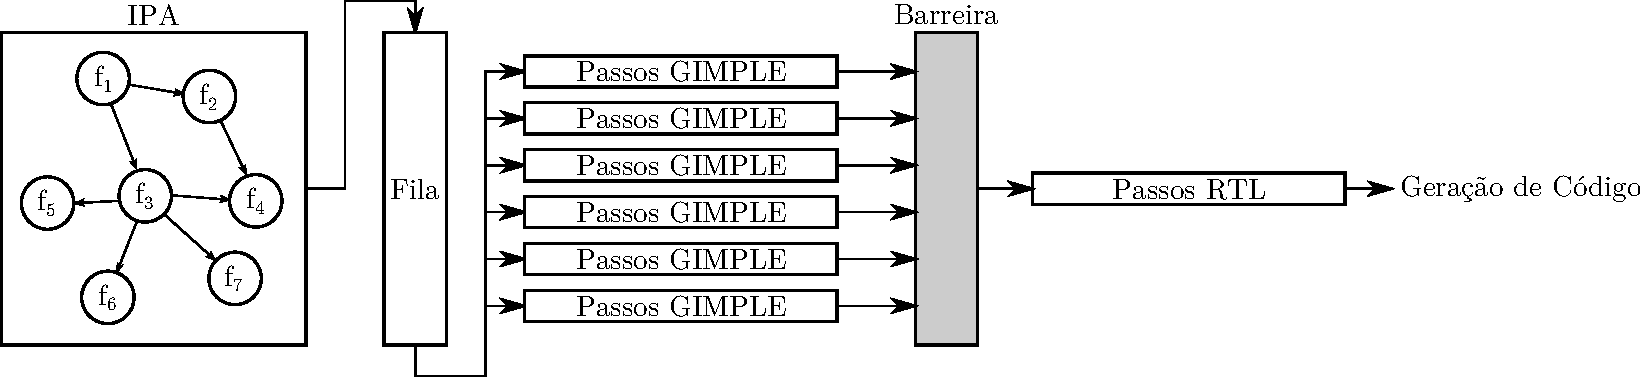
\includegraphics[width=\textwidth]{paralelizacao.pdf}
 \caption{Per-function parallelization schematic}
 \label{fig:paralelizacao}
\end{figure}

Since GCC is a huge software, we only selected a subset of the optimization
passes for this thread-based approach, which we selected the GIMPLE passes.
We begin by splitting the pass engine into explicitly three steps: IPA transformation,
GIMPLE, and RTL, and we made sure that we could run all IPA transformations first on
every function, then all GIMPLE passes in every function, then all RTL passes in
every function; as opposed to the previous mode that applied every optimization
to a single function before proceding to the next function. Figure
\ref{fig:intraprocedural_sketch} illustrates how this process was before our
change, and \ref{fig:intraprocedural_sketch_after} illustrates our modifications.

\begin{figure}[ht]
	\centering
	\begin{lstlisting}[
		language=pseudocode,
		style=pseudocode,
		style=wider,
		functions={},
		specialidentifiers={graph},
		]
graph* g = build_callgraph ();
ipa_perform_analysis (g);
function* cfun;
FOR_EACH_FUNCTION (g, cfun) {
  cfun->expand ();
}
	\end{lstlisting}
\caption{Sketch of GCC aplying the intraprocedural optimizations}
\label{fig:intraprocedural_sketch}
\end{figure}


\begin{figure}[ht]
	\begin{center}
	\begin{lstlisting}[
		language=pseudocode,
		style=pseudocode,
		style=wider,
		functions={},
		specialidentifiers={graph},
		]
graph* g = build_callgraph ();
ipa_perform_analysis (g);
function* cfun;
working_set ws;

FOR_EACH_FUNCTION (g, cfun) {
  cfun->expand_ipa ();
}

ws.spawn_threads (expand_gimple):

FOR_EACH_FUNCTION (g, cfun) {
  ws.insert_work (cfun);
}
ws.join()

FOR_EACH_FUNCTION (g, cfun) {
  cfun->expand_rtl ();
}
	\end{lstlisting}
	\end{center}
\caption{Sketch of GCC aplying the intraprocedural optimizations after our changes}
\label{fig:intraprocedural_sketch_after}
\end{figure}

After that, we chose to parallelize the GIMPLE passes. We chose GIMPLE first because
it affects every target architecture supported by GCC, whereas RTL would require
adjustement to every target architecture. For this to work minimally, we had to
insert locks to several points in the compiler -- which is the main issue with
this approach -- that we discuss below.

\begin{subsection}{Global Variables}

The first major problem was the abuse of global variables in GCC, and the lack
of replicability of critical data structures that are necessary for compiling a
function. For instance, the current function pointer (cfun) is a global
variable used in almost every intraprocedural pass in GCC, although the pass
engine itself supports passing the function which must be compiled. Other
structures required replication across the threads, which we used the C11
Thread Local Storage feature (\textit{\_\_thread}).

Then there were the problems with global variables in most passes, which used
global variables to avoid passing them down into the callchain. This issue can
be fixed by wrapping these variables inside a class and instantiate them on the
pass execution.

\end{subsection}

\begin{subsection}{Memory Pools}

Memory pools are data structures that allocate several objects of the same type
in chunks to avoid calls to the \texttt{malloc()} function, and to ensure that data is
always aligned. This serves both as optimization and to avoid memory leaks, as
one can free the entire pool at once. 

Memory pools were implemented in GCC as a class that all points to one
singleton Memory Allocator object, which carries the memory allocation and
therefore had a serious race condition when threads tried to allocate and
deallocate memory pools. One thread could release a pool to which other threads
held pointers to, resulting in references to invalid memory, or typical race
conditions in this structure with counters, which need to be increased and
decreased as chunks of objects are allocated and released. 
As the data structure is required by other threads later in the compilation,
which is still carried by a single thread in the current state of this project,
our first try was to implemented a Threadsafe Memory Pool allocator, which
locks a mutex each time memory is allocated or released and annotates the
thread ID on each chunk. Therefore, when memory is released, the thread only
releases the chunk they currently own. This approach made the compilation slow,
and the GCC tests failed due to time concerns. Therefore, another strategy was
designed. 

The second approach was to use a distributed memory pool. Each thread holds one
memory pool, and as a result, there is no need for locking when allocating and
releasing the chunks. This also guarantees that one thread does not release the
contents of another thread, as they have no access to pools that belongs to
other threads. However, this leads to an issue, as the data is required by
another thread later in the compilation. The solution was to implement a pool
merge feature, which merges two memory pools upon request. Since memory pools
are implemented as a linked list, the merge feature could be implemented in
$O(1)$, although the current implemented algorithm requires $O(n)$. The reason for
this is that the memory pool currently uses a single-headed linked list, and it
needs to be refactored into a double-headed linked list. 

All memory pools touched by GIMPLE Intra Process Optimizations, except one,
were refactored with this approach, and the merge feature was used only in
those memory pools which were required. The only pool which was not refactored
using this approach was the Euler Transversal Forest data structure
(et-forest.c), simply because the compiler crashes when the strategy is
employed here. The reason for this must still be investigated.

\end{subsection}

\begin{subsection}{Garbage Collector}

GCC has an internal garbage collector, which is a reference counter of objects.
Objects that are watched by the garbage collector are declared with the GTY(())
annotation, and we can not simply use C11 thread annotation, as it is not
supported by the Garbage Collector. Our approach is to either insert locks in
these variables or move them inside the function object.

We fixed the issue with the Garbage Collector by ensuring that memory
allocation at this point is serialized, and disabled any memory collection when
the program is running in multi-threaded mode. This is not necessary when
multi-thread is supported by the Garbage Collector.

\end{subsection}

\begin{subsection}{Memory Address to Symbol Conversion}

GCC uses a cache to keep tracks of memory address allocated to symbols (in
\texttt{tree-ssa-address.c}) and it is used to check if an address is part of a symbol
(i.e., access to an array). This cache array is marked to be watched by the
garbage collector, therefore we lock this structure every time this array has
to be accessed. Research is needed to evaluate how much this lock impacts
performance, and if there is a better way of handling this situation. 

\end{subsection}

\begin{subsection}{Integer to Tree Node Hash}

In \texttt{tree.c}, there is a hash table used to avoid reconstruction of tree nodes
that represent integer constants. This hash is also marked to be watched by the
Garbage Collector, and therefore we used a simple lock to this structure every
time this hash is accessed. This approach may not be the best if the cost of
locking and hashing becomes greater than recreating the tree node. Therefore
research is also needed here. 

\end{subsection}

\begin{subsection}{The rtl\_data Structure}

GCC uses a single instance of rtl\_data class, representing the current function
being compiled in RTL. This should not be a problem as RTL expansion
and optimization phase is still single-threaded. However, there are GIMPLE
passes which calculate instruction costs in RTL mode to decide how the function
will be optimized. This access the rtl\_data singleton and therefore exposes a
race condition that needs to be solved. To fix this issue, we have either to
replicate this structure, which is necessary to parallelize the intraprocedural
RTL optimizations, or fix the GIMPLE pass so that it does not depends on
instruction costs. 

\end{subsection}

\begin{subsection}{Results}

Here we present our current performance results by parallelizing the GIMPLE
Intra Process Optimizations. It must be highlighted that this project still had
race conditions, which we discuss later, and further, some locks can be
removed, as data structure can be duplicated and the garbage collector could be
deserialized.

Here we compile the file \texttt{gimple-match.c}, which is the biggest file in
the GCC project. The computer used in this Benchmark had an Intel(R) Core(TM)
i5-8250U CPU, with 8Gb of RAM.  Therefore, this computer had a CPU with 4 cores
with Hyperthreading, resulting in 8 virtual cores. All points are the mean of
30 samples, and the confidence interval to the populational mean was
suppressed, as the standard deviation was fairly low. 

Figure \ref{fig:parallel_gimple} below shows our results before and after Intra
Procedural GIMPLE parallelization. In this figure, we can observe that the time
elapsed in this part dropped from 7 seconds to around 4 seconds with 2 threads
and around 3 seconds with 4 threads, resulting in a speedup of 1.72x and 2.52x,
respectively. Here we can also see that using Hyperthreading did not impact the
result. This result was used to estimate the improvement in RTL
parallelization.

Next, Figure \ref{fig:parallel_real} shows this results when compared with the
total compilation time. Here we can see that there is a small improvement of
10\% when compiling this file.

However, since the same approach can be used to parallelize RTL, we can
estimate a speedup of 1.61x in GCC when it gets parallelized by using the
speedup information obtained in GIMPLE, as illustrated in Figure
\ref{fig:parallel_estimate}.

\begin{figure}[ht]
 \centering
 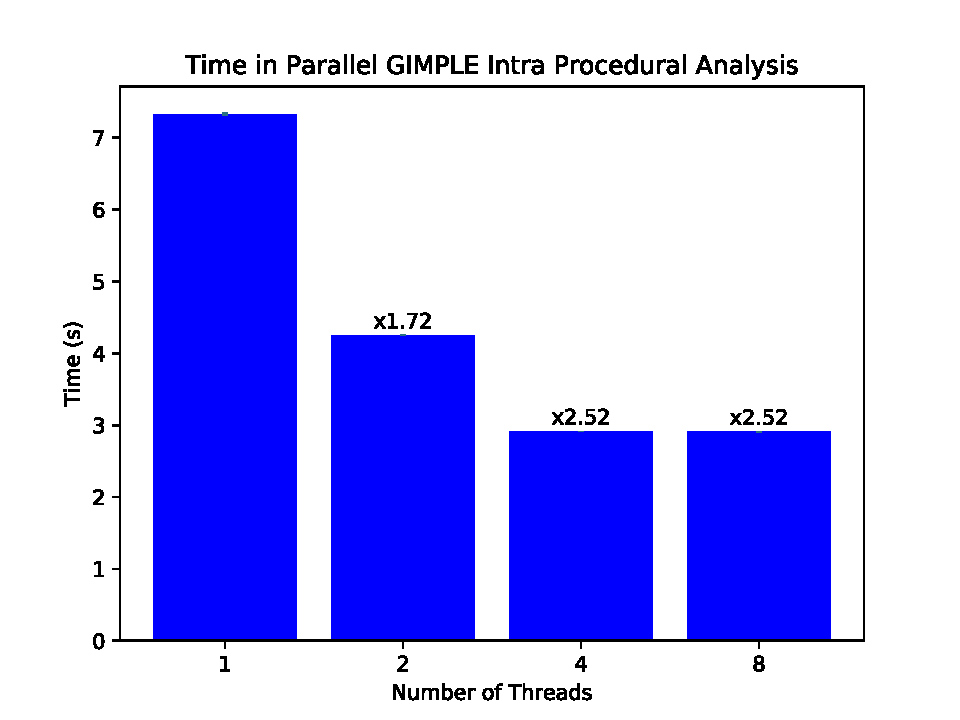
\includegraphics[scale=0.7]{gimple_parallel.pdf}
 \caption{Results of parallelizing GIMPLE passes}
 \label{fig:parallel_gimple}
\end{figure}

\begin{figure}[ht]
 \centering
 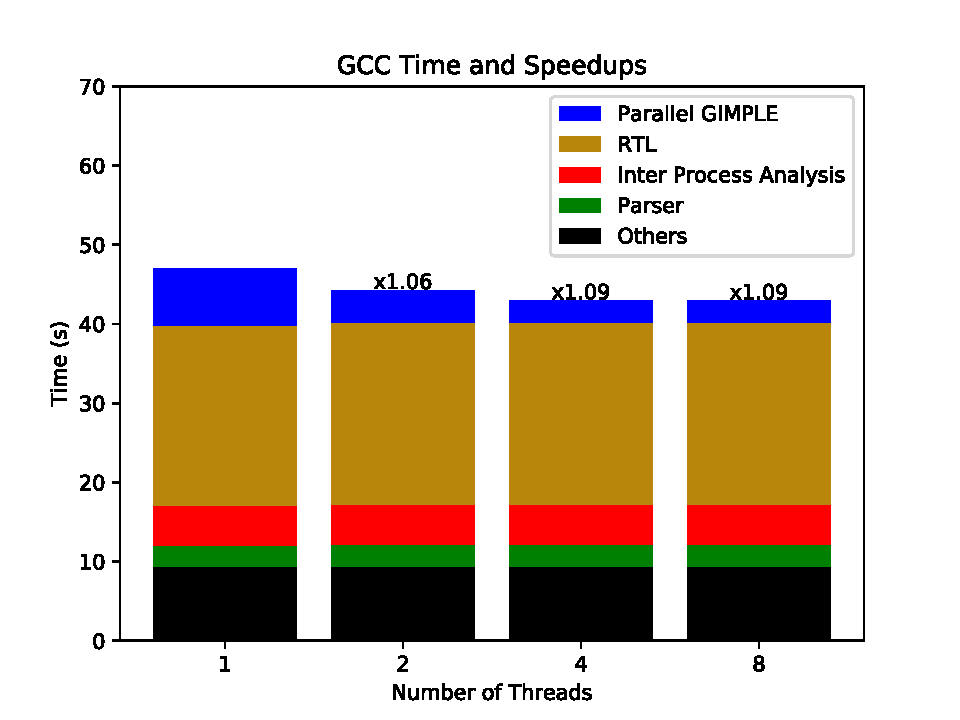
\includegraphics[scale=0.7]{real.pdf}
 \caption{Speedup in total compilation time when parallelizing GIMPLE}
 \label{fig:parallel_real}
\end{figure}

\begin{figure}[ht]
 \centering
 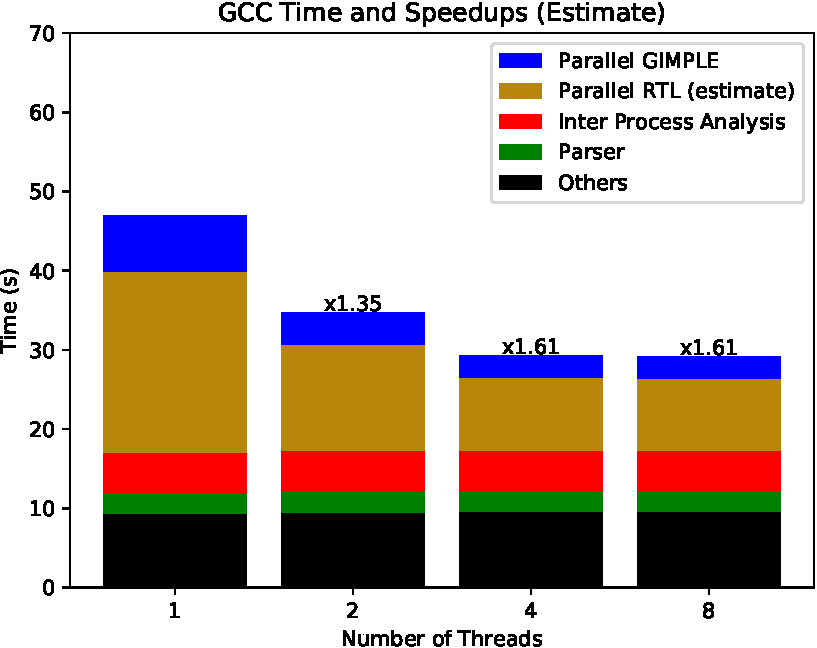
\includegraphics[scale=0.7]{gcc_estimate.pdf}
 \caption{Estimate parallel time when also parallelizing RTL}
 \label{fig:parallel_estimate}
\end{figure}

\end{subsection}

\begin{subsection}{Feasibility Discussion}

We have presented that it is possible to parallelize parts of the compiler for
parallel execution. However, using threads on an already fully developed
compiler may not be feasible from the point of development itself because of
its complexity.

The main reason is that incremental parallelizing them is hard. The test suite
does not help on that, once they are very small programs designed to test a
certain aspect of the compiler, meaning that there is not enough stress test.
There are programs such as Helgrind and ThreadSanitizer which improves our job,
but even then, we reach a point where the race condition window is so small
that even those tools fail to detect them. There is no alternative left than
indeed understanding the code and figuring out on our own what is causing the
race condition. This certainly is the problem not only in compilers but in
large software in general.

With this in mind, perhaps the best approach is to go using a process-based
approach rather than threads, which we discuss in the next section.

\end{subsection}

\end{section}

\begin{section}{Modifying LTO for parallel file compilation}\label{sec:parallel_lto}

As presented in Section \ref{lto_section}, LTO was created to allow
cross-module optimizations in programs, and has a serial part (WPA), imposing a
compilation bottleneck on manycore machines. On the other hand, \emph{classical
compilation} scheme can not partition its TU for parallel compilation, which
can also be a bottleneck for the compilation if it is too large.  The latter
issue, however, can be solved by transplanting the LTO partitioner to the
\emph{classical compilation} scheme and making it work \textit{without} having
the context of the \textit{entire} program. We show that this transplant it is
possible by implementing it in GCC.

Here we present our approach regarding parallel compilation using process. For
that, we do simple modifications to the LTO engine.  Our approach differs from
LTO mainly in how we handle the IPA.  LTO handles these optimizations with the
context of the whole program, while our approach will only have the context of
the original TU.  This allows optimizations as good as they are in the
\emph{classical compilation} scheme while benefiting from the extra parallelism
opportunity available in the LTO's LTRANS stage.

In this section, we will first discuss the internals of some parts of GCC,
which we had to modify for our implementation to work. In Subsection
\ref{sec:gcc_driver}, we present an important piece of the compiler from the
User Experience perspective: the \texttt{gcc} \textit{driver}. Then, in
Subsection \ref{sec:lto_partitioner} we present a short algorithm for making
the LTO partitioner work for our proposal. In Subsection
\ref{sec:partition_mask} we present a necessary change we had to do in our work
about how partitions are applied in GCC. In
Subsection \ref{sec:name_clash_resolution}, we explain how we solved the issue
of private symbols with the same name being promoted to global.
Then in Subsection \ref{sec:integration_jobserver}, we present an optional part
of our work about communicating with the GNU Make Jobserver to keep track of
used processors. And finally, we discuss why our proposal is still compatible
with the Reproducible Builds project in Subsection \ref{sec:repro_builds}.

\begin{subsection}{The \texttt{gcc} Driver}\label{sec:gcc_driver}

A large program can be written in several languages, with each of them having
its own compiler. As stated in Section \ref{sec:motivation}, a compiler
translates a program from a language $A$ to another language $B$.
In GCC, it translates several languages to assembly
of some architecture (\textit{e.g.} x86). This means that
encapsulating code in object files, or linking these files in an executable, are
not tasks of the compiler. However, the user can launch \texttt{gcc -o binary
file.c} and get a working binary. That is because the binary \texttt{gcc} is
a \textit{driver}, and it will launch the
necessary programs for the user. In fact, this line launches three programs,
as illustrated in Fig. \ref{fig:gnu_toolchain}.

Therefore, if we want our changes do not break the building scripts
(\textit{e.g.}, Makefile) used by most projects -- which is mostly launching
\texttt{gcc file.c -c} that creates an object file \texttt{file.o} -- we must
ensure that we create a single object file for each file, not multiple, as does
the LTO partitioner. Fortunately, we can rely on GNU \textit{ld} partial linking
for merging objects file into one. Therefore, the solution to this problem is:
\begin{enumerate}
	\item Patch the LTO \textit{partitioner} to communicate the location of
	each created assembly file (.s) to the \textit{driver}. This can be
	done by passing a hidden flag \texttt{-fadditional-asm=<file>}
	by the driver to the partitioner, which the last will write to. This file can also
	be replaced with a Named Pipe for better performance if needed.

	Then, the partitioner checks if this flag has been passed to the compiler.
	If yes, then a \textit{compatible version} of the driver is installed. If
	the partitioner decides to partition the TU, it should \textit{retarget}
	the destination assembly file and write the retargeted name to the
	communication file.

	\item Patch the driver to pass this hidden flag to the
	\textit{partitioner}, and also to check if this file exists. If not, this means
	that either the compiler is incompatible or it has chosen not to partition
	the TU. In the first case, the driver should call the assembler to every
	assembly file generated, and call the linker to generate the expected
	final object file. In the second case, simply fallback to the previous
	compilation logic.
\end{enumerate}

Fig. \ref{fig:gnu_toolchain_patched} illustrates the code flow after these
changes.  The execution starts in the highlighted node \textit{gcc}, which
calls the compiler (cc1) with the necessary flags to establish a communication
channel among the parts. The compiler then will partition the TU and forks
itself into several child processes, one for each partition.

Once multiple processes are created, the compiler will communicate its output
.s file, and the driver then will launch the assembler (\textit{as}) to
generate several object files, and then launch the linker (\textit{ld}) to
merge them all into a single object file.

\begin{figure}
\tikzstyle{block} = [rectangle, draw, fill=white,
    text width=6em, text centered, rounded corners, minimum height=2em]
\tikzstyle{line} = [draw, -latex]

\makebox[\textwidth][c]{
\scalebox{0.8}{
\begin{tikzpicture}[node distance = 3cm, auto]
    % Place nodes
    \node [block]                      (cc1_1) {cc1};
    \coordinate [right= of cc1]          (c);
    \node [block, right= of c,fill={rgb:black,1;white,2}]        (driver1) {gcc};
    \node [block, above= of c]                      (cc1_2) {cc1};
    \node [block, below= of c]                      (cc1_3) {cc1};
    \coordinate [above= of driver1]          (c2);
    \coordinate [below= of driver1]          (c3);
    \node [block, right= of c2]      (as2) {as};
    \node [block, right= of c3]      (as3) {as};
    \node [block, right= of driver1]       (ld) {ld};
    \coordinate [left= of cc1]          (fonte);
    \coordinate [right= of ld]    (bin);

    % Draw edges
    \draw[->]    (driver1.west)    -- (cc1_1.east) node[midway, above] {\texttt{-fadditional-asm=<file>}};
    \draw[->]    ([xshift=+0.5cm]cc1_2.south) -- ([xshift=-0.5cm]driver1.north) node[midway, above, sloped] {Generates .s file};
    \draw[->]    ([xshift=+0.5cm]cc1_3.north) -- ([xshift=-0.5cm]driver1.south) node[midway, above, sloped] {Generates .s file};

    \draw[->]    (cc1_1.north)    -- ([xshift=-0.5cm]cc1_2.south) node[midway, above, sloped] {Forks};
    \draw[->]    (cc1_1.south)    -- ([xshift=-0.5cm]cc1_3.north) node[midway, above, sloped] {Forks};

    \draw[->]    ([xshift=+0.5cm]driver1.north)  -- (as2.south) node[midway, above, sloped] {Assemble received .s};
    \draw[->]    ([xshift=+0.5cm]driver1.south)  -- (as3.north) node[midway, above, sloped] {Assemble receibed .s};
    \draw[->]    (driver1.east)  -- (ld.west) node[midway, above, sloped] {Links};

%    \draw[->]    (cc1.east)    -- (as.west)       node[midway, above] {Assembler File};
%    \draw[->]    (cc1.east)    -- (as.west)       node[midway, above] {Assembler File};
%
%    \draw[->]    (cc1.east)    -- (as.west)       node[midway, below] {(.s)};
    \draw[->]    ([xshift=+0.5cm]as2.south)     -- (ld.north)       node[midway, above, sloped] {Object File};
    \draw[->]    ([xshift=+0.5cm]as3.north)     -- (ld.south)       node[midway, below, sloped] {Object File};
%    \draw[->]    (fonte.west)  -- (cc1.west)      node[pos=0, above] {Source File};
%    \draw[->]    (fonte.west)  -- (cc1.west)      node[pos=0, below] {(.c)};
    \draw[->]    (ld.east)     -- (bin.west)      node[pos=1, above] {\texttt{file.o}};
\end{tikzpicture}
}
}%
\caption{Interaction between the \textit{driver}, the \textit{compiler}, and other tools
after our changes}
\label{fig:gnu_toolchain_patched}
\end{figure}

\end{subsection}

\begin{subsection}{Adapting the LTO partitioner}\label{sec:lto_partitioner}

In GCC, a TU is represented as a callgraph. Every function, global variable, or
clones (which may represent a function to be inlined) is represented as nodes
in a callgraph. If there is a function call from $f$ to $g$, or there is a
reference to a global variable $g$ in $f$, then there is an edge from $f$ to
$g$. This means that TU partitioning can be represented as a \emph{graph
partitioning} problem.

When LTO is enabled and GCC is in the WPA stage, the body of these nodes
is not present, just a \textit{summary} of them (\textit{e.g.} the size
in lines of code it had). This is done to save memory. However,
when LTO is disabled, the function body is present, resulting
in some assertion failures, which were fixed after some debugging.

Then comes the partitioner algorithm \textit{de facto}. In LTO, GCC tries to
create partitions of similar size, and always try to keep nodes together. The
heuristic used by the original partitioner runs in linear time, and because of
that its code is quite complex. This resulted in a difficult process of finding
and solving the issues causing a partitioning failure, and therefore, we
decided to design a new partitioning algorithm for this project.

This partitioning algorithm works as follows: for each node, we check if it
is a member of a COMDAT \citep{comdat} group, and
merged it into the same partition. We then propagate outside of this COMDAT group;
checking for every node that may trigger the COMDAT to be copied into other
partitions and group them into the same partition. In practice,
this means to include every node hit by a Depth-First
Search (DFS) from the group to a non-cloned node outside of the group.
Fig. \ref{fig:comdat_frontier} represents a sketch of this process.

\begin{figure}
\centering
	 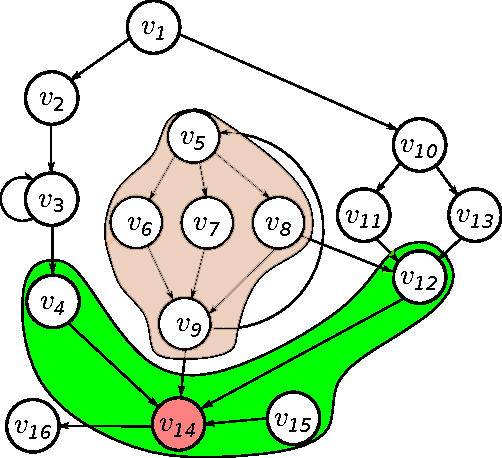
\includegraphics[scale=0.7]{figuras/comdat_frontier.pdf}
	  \caption{Example of callgraph, in beige being represented the COMDAT group,
	  in green the COMDAT frontier, and in red the cloned nodes.}
	  \label{fig:comdat_frontier}
\end{figure}

At first, we also did this process for private functions to avoid
promoting them to public, once external access would be necessary if they go
into distinct partitions. However, results showed that this has a strong
negative hit in any parallelism opportunity.

For grouping the nodes together,
we used a Union Find with Path Compression, which yields an attractive
computational complexity of $O(E + N \lg^*N)$ to our partitioner, where $N$ is the
number of nodes and $E$ is the number of edges in the callgraph \citep{feufiloff}.

Once the partitions are computed, we need to compute its \textit{boundary}.
If function $f$ calls $g$, but they were assigned into distinct partitions,
then we must include a version of $g$ in $f$'s partitions without its body,
then check if $g$ is a private function. If yes, then $g$ must be promoted
to a public function. There is also extra complexity if a version of $g$
is marked to be inlined in $f$, which means that its body has to be
streamed somehow. Fortunately, most of this logic is already present
in LTO and we could reuse them. However, some issues were found
when handling inline functions and global variables marked as part
of the boundary. First, some functions marked to be inlined into 
functions inside the partition were incorrectly marked to be removed.
Second, being variables marked as in the boundary (and therefore
not in the partition) not being correctly promoted to external. The reason
for these issues was hard to find the reason of, but easy to fix.

Furthermore, there were some issues concerning how GCC handles
partitions, which we discuss in the next subsection.

\end{subsection}

\begin{subsection}{Applying a Partition Mask}\label{sec:partition_mask}

Once partitions are computed, the only presented way to apply it
(\textit{i.e.}, remove every unnecessary node from the TU) was to reload the
compiler and let it load the phony object files. The issue is that these
objects are not available in our project because we are not running in LTO
mode. We developed another method for this.
We used the Unix \textit{fork} function to spawn a child process, and then
we implemented our own method to apply the partition without having to load
these phony object files. Fortunately, this consisted
of four cases:
\begin{itemize}
	\item \textit{Node is in partition}: nothing has to be done.
	\item \textit{Node is in boundary, but keep its body}: we mark that this function
	is available in other partitions, but we do not release its body or
	data structures.
	\item \textit{Node is in boundary}: we mark this mode as having its body removed,
	but we never actually remove it. This is because the node may share the
	body contents with another node in the partition. We then remove
	every edge from its functions to its callees, all references to variables,
	the content of the Dominator Tree, and also its Control-Flow Graph. This
	is now a function which this partition only know that it exists.
	\item \textit{Node not in boundary}: we remove the node and all its content.
\end{itemize}

After this, it retargets the output assembly file to another file private to
this partition and writes a pair (\textit{partition number, path to file}) into the
communication file, which the driver will read in the future. The partition
number is important to guarantee that the build is reproducible, as we will
discuss later.

It is also important that some early step in the compiler does not emit assembly
too early, such as the issue with the gimplifier in GCC, or else the output
file will be incomplete. We had to fix the gimplifier to avoid that.

Once the partition is applied to the child process, and the output file has
been communicated to the driver, it can continue with the compilation. It
should be running in parallel now by the number of partitions.

\end{subsection}

\begin{subsection}{Name Clash Resolution}\label{sec:name_clash_resolution}

In LTO, if there are two promoted symbols to global with the same (mangled) name, a
straightforward way to fix that is to increment a counter for each clashed
symbol. This is possible because LTO has the context of the entire program,
which we do not. Therefore, we need another way of fixing it.

Two naive approaches would be to select a random integer and append to the
function's name, or append the memory address of the function object to the
function's name.  Both of them breaks bootstrap \citep{bootstrap}, the first
because output functions will have distinct names on every new compilation. The
second because stage 1 compiles with \texttt{-O0} and stage 2 with
\texttt{-O2}, which changes the memory address of the functions between these stages.

Our solution is to use a crc32 hash of the original file and append it to the
function's name.  There is still a tiny probability of name clash with this
approach, however, we did not find any on our tests.

\end{subsection}

\begin{subsection}{Integration with GNU Make Jobserver}\label{sec:integration_jobserver}

GNU Make can launch jobs in parallel by using \texttt{make -j}.  To
avoid unnecessary partitioning and job creation when the CPU is at 100\% usage,
we have also implemented an integration mechanism with GNU Jobserver
\citep{posixjobserver}.  The implementation is simple: we query the server for
an extra token. If we receive the token, then it means that some processor is
available, and we can partition the TU and launch jobs inside the compiler.
Else, the processor workload is full, and it may be better to avoid
partitioning altogether.

However, for a program to be able to communicate with the jobserver, it should
be launched with a prepended \texttt{+} character (\textit{e.g.} $\texttt{+gcc
-c file.c}$), and therefore it is not so straightforward to use this mode on
existing projects.

\end{subsection}

\begin{subsection}{Relationship with Reproducible Builds}\label{sec:repro_builds}

One interesting point of Open Source is that it can be verified by everyone.
However, very often these projects are distributed in a binary form to the
users, removing from them the burden of this process. But nothing avoids that a
malicious developer modifies the codebase \textit{before} the distribution
(\textit{e.g.} inserting a backdoor), and claiming that he/her got a distinct
binary because his/her system is different from the user.

The Reproducible Builds project aims to solve that issue by providing a way to
reproduce the released binary from its source. Some software needs to
be patched to work with Reproducible Builds, for instance,
to not contain some kind of build timestamp, and so on. A build
is called \textit{reproducible} if given the same source code and build
instructions, anyone can recreate a bit-perfect version of the distributed
binary \citep{reproducible_builds}.

To keep compatibility with this project, we must ensure that our compiler
always outputs the same code with a given input. The input is not only
the source file itself but also the flags passed to it.

We claim that our modification still supports the Reproducible Builds because
of the following reasons:

\begin{itemize}
	\item No random information is necessary to solve name clashing.
	\item Given a number of jobs, our partitioner will always generate
	the same number of partitions for a certain program, always with the same content.
	\item Partial Linking is always done in the same order. To ensure that,
	we communicate to the driver a pair (\textit{partition number, path to file}),
	and we sort this list using the partition number as the key.
	\item No other race conditions are introduced, as we rely on the quality of
	the LTO implementation of the compiler.
\end{itemize}

However, there is one point of concern, which is the Jobserver Integration.  If
the processor is already in 100\% usage, we avoid partitioning at all and
proceed with sequential compilation. This certainly changes accordingly to the
processor usage of the machine during the build, therefore the build is not
guaranteed to be reproducible if this option is enabled. This is not an issue
if the number of jobs is determined beforehand.

\end{subsection}

\begin{subsection}{Methods}\label{sec:methods}

We ensure the correctness of our changes by running these tests with 2, 4, 8
and 64 parallel jobs, with minimum partitioning quota of $10^3$ and $10^5$
instructions:
\begin{enumerate}
\item Bootstrapping GCC.
\item Ensure that the GCC testsuite was passing.
\item compiling random programs generated with \textit{csmith} \citep{csmith}
and ensure that the correct result was found.
\end{enumerate}

For the time measurements, all points represent the average of collected
samples, with errorbar representing a $95\%$ confidence interval.
Our test files consisted of preprocessed source files from GCC, which compiles
without external includes. We collected $n = 15$ samples for every one of these
files. For the projects, we collected $n = 5$ samples because compilation is a
computer intensive task. We made sure that in every test, \texttt{-g0} was passed
for fairness, once there is a bug in our branch regarding debug symbols of
nodes in other partitions.

For the power usage measurement, we used the builtin AMD \texttt{fam15h\_power}
sensor available in the Opteron CPU \citep{fam15h}.

Tests were mainly executed in two computers, which are represented
in Table \ref{table:machines}. The graphic caption specifies where the test
was run.

\begin{table}[]
\centering
\begin{tabular}{c|c|c|c|c|}
\cline{2-5}
                                      & Number of Cores & Number of Threads & RAM                                                    & Storage Device \\ \hline
\multicolumn{1}{|c|}{Core-i7 8650U}   & 4               & 8                 & \begin{tabular}[c]{@{}c@{}}8Gb\end{tabular} & SSD       \\ \hline
\multicolumn{1}{|c|}{4x Opteron 6376} & 32              & 64                & \begin{tabular}[c]{@{}c@{}}252Gb\end{tabular}   & HDD       \\ \hline
\end{tabular}
\caption{Machine specification of tests}
\label{table:machines}
\end{table}


The version of GCC used in the tests is available in the \texttt{autopar\_europar\_2021}
branch of \texttt{git://gcc.gnu.org/git/gcc.git}, with hash \texttt{e2da2f7205}.

\end{subsection}

\begin{subsection}{Results}\label{sec:results}

We first highlight our best results in Table \ref{table:files}. On this table,
the autogenerated column means that this file is compiled to C++, and then compiled
into assembly by GCC. We managed speedups of up to a $2.4\times$ on Core-i7 when
compiling individual files with 8 threads, and up to $3.53\times$ on Opteron 6376 when
with 64 threads. Fig. \ref{fig:gcc_all_files} shows the results
of all files in GCC. Here we can see that for files with $\textit{Number of Instructions} >
1 \times 10^5$, we have mostly significant improvements.

We will now discuss how our proposed changes impact the overall compilation
time of some projects. For this, we run experiments compiling
the Linux Kernel 5.19.6, Git 2.30.0, the GCC version mentioned in
Section \ref{sec:methods} with and without bootstrap enabled, and JSON C++, with
commit hash \texttt{01f6b2e7418537}. We have only enabled jobserver integration
in GCC and Git, because it is necessary to modify an absolute large number
of Makefiles to do so (for instance, Linux has 2597 Makefiles).

In Fig. \ref{fig:gcc_projects} we show our results. We can observe a near
$35\%$ improvement when compiling GCC with bootstrap disabled, $25\%$ when
bootstrap is enabled, and $15\%$ improvement when compiling Git compared to
\texttt{make -j64} alone. Our jobserver implementation also squeezed a small
improvement in GCC compilation, but showed a massive slowdown in Git. This is
because Jobserver integration has interprocess communication cost
with Make, which is a problem if the size of the partitions is small.  These
tests were executed with 64 Makefile jobs and 8 threads inside the compiler.
Other than this, we seen no significant speedup or slowdown in these other
projects.

We can explain our results regarding GCC by looking by comparing Figures
\ref{fig:analysis_classical} and \ref{fig:analysis_classical_parallel}. On
Figure \ref{fig:analysis_classical}, we have the classical compilation scheme,
which has some bottlenecks due to high time-consuming files. When our changes
are applied and the compiler is running in parallel (Figure
\ref{fig:analysis_classical}), we see a reduction of compilation time on those
files. Therefore, by compiling files in parallel, we can reduce the time
required to compile those files when we have available free CPU cores.

Furthermore, we also observe a reduction in power consumption when using this
mode, which is displayed in Figure \ref{fig:power}. This may be extra useful for Continuous Integration systems, which
may compile the same software from scratch several times a day.

\begin{table}[]
\makebox[\textwidth][c]{
\begin{tabular}{l|c|c|c|c|c|c|c}
\cline{2-7}
                                       & \multicolumn{3}{c|}{Core-i7}     & \multicolumn{3}{c|}{Opteron 6376}                                                                & \multicolumn{1}{l}{}               \\ \hline
\multicolumn{1}{|l|}{File}             & Sequential & 8 Threads & Speedup & \multicolumn{1}{l|}{Sequential} & \multicolumn{1}{l|}{64 Threads} & \multicolumn{1}{l|}{Speedup} & \multicolumn{1}{c|}{Autogenerated} \\ \hline
\multicolumn{1}{|l|}{gimple-match.c}   & $76s$        & $31s$       & $2.4\times$     & $221s$                            & $66s$                             & $3.32\times$                         & \multicolumn{1}{c|}{yes}           \\ \hline
\multicolumn{1}{|l|}{insn-emit.c}      & $23s$        & $10s$       & $2.25\times$    & $97s$                             & $37s$                             & $3.53\times$                         & \multicolumn{1}{c|}{yes}           \\ \hline
\multicolumn{1}{|l|}{tree-vect-stmt.c} & $11s$        & $5s$        & $2.14\times$    & $32s$                             & $13s$                             & $2.46\times$                         & \multicolumn{1}{c|}{no}            \\ \hline
\end{tabular}
}
\caption{Speedup of highlighted files}
\label{table:files}
\end{table}

\begin{figure}
\centering
	 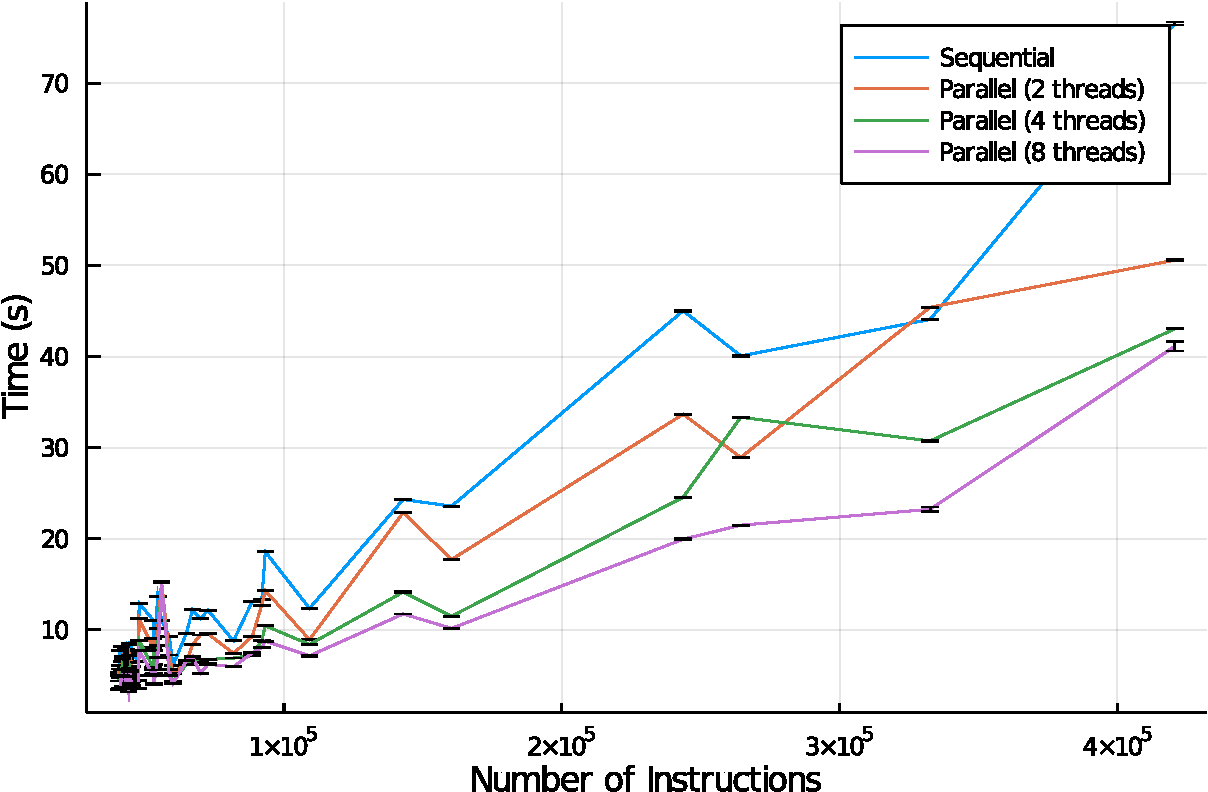
\includegraphics[scale=0.6]{figuras/times-insns-crop.pdf}
	  \caption{Compilation of each file with 1, 2, 4, and 8 threads on
	  Core-i7}
	  \label{fig:gcc_all_files}
\end{figure}

\begin{figure}
\centering
	 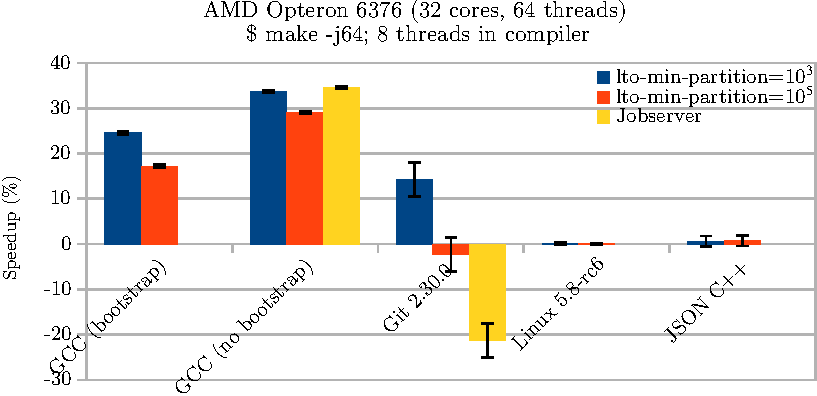
\includegraphics[scale=0.85]{figuras/experiment_projects_new-crop.pdf}
	  \caption{Compilation of some projects with 64 Makefile jobs and 8 threads in compiler in Opteron 6376}
	  \label{fig:gcc_projects}
\end{figure}

\begin{landscape}
%\begin{figure}[ht]
 \vspace*{-2cm}%
 \noindent%
 \hspace*{-2cm}%
    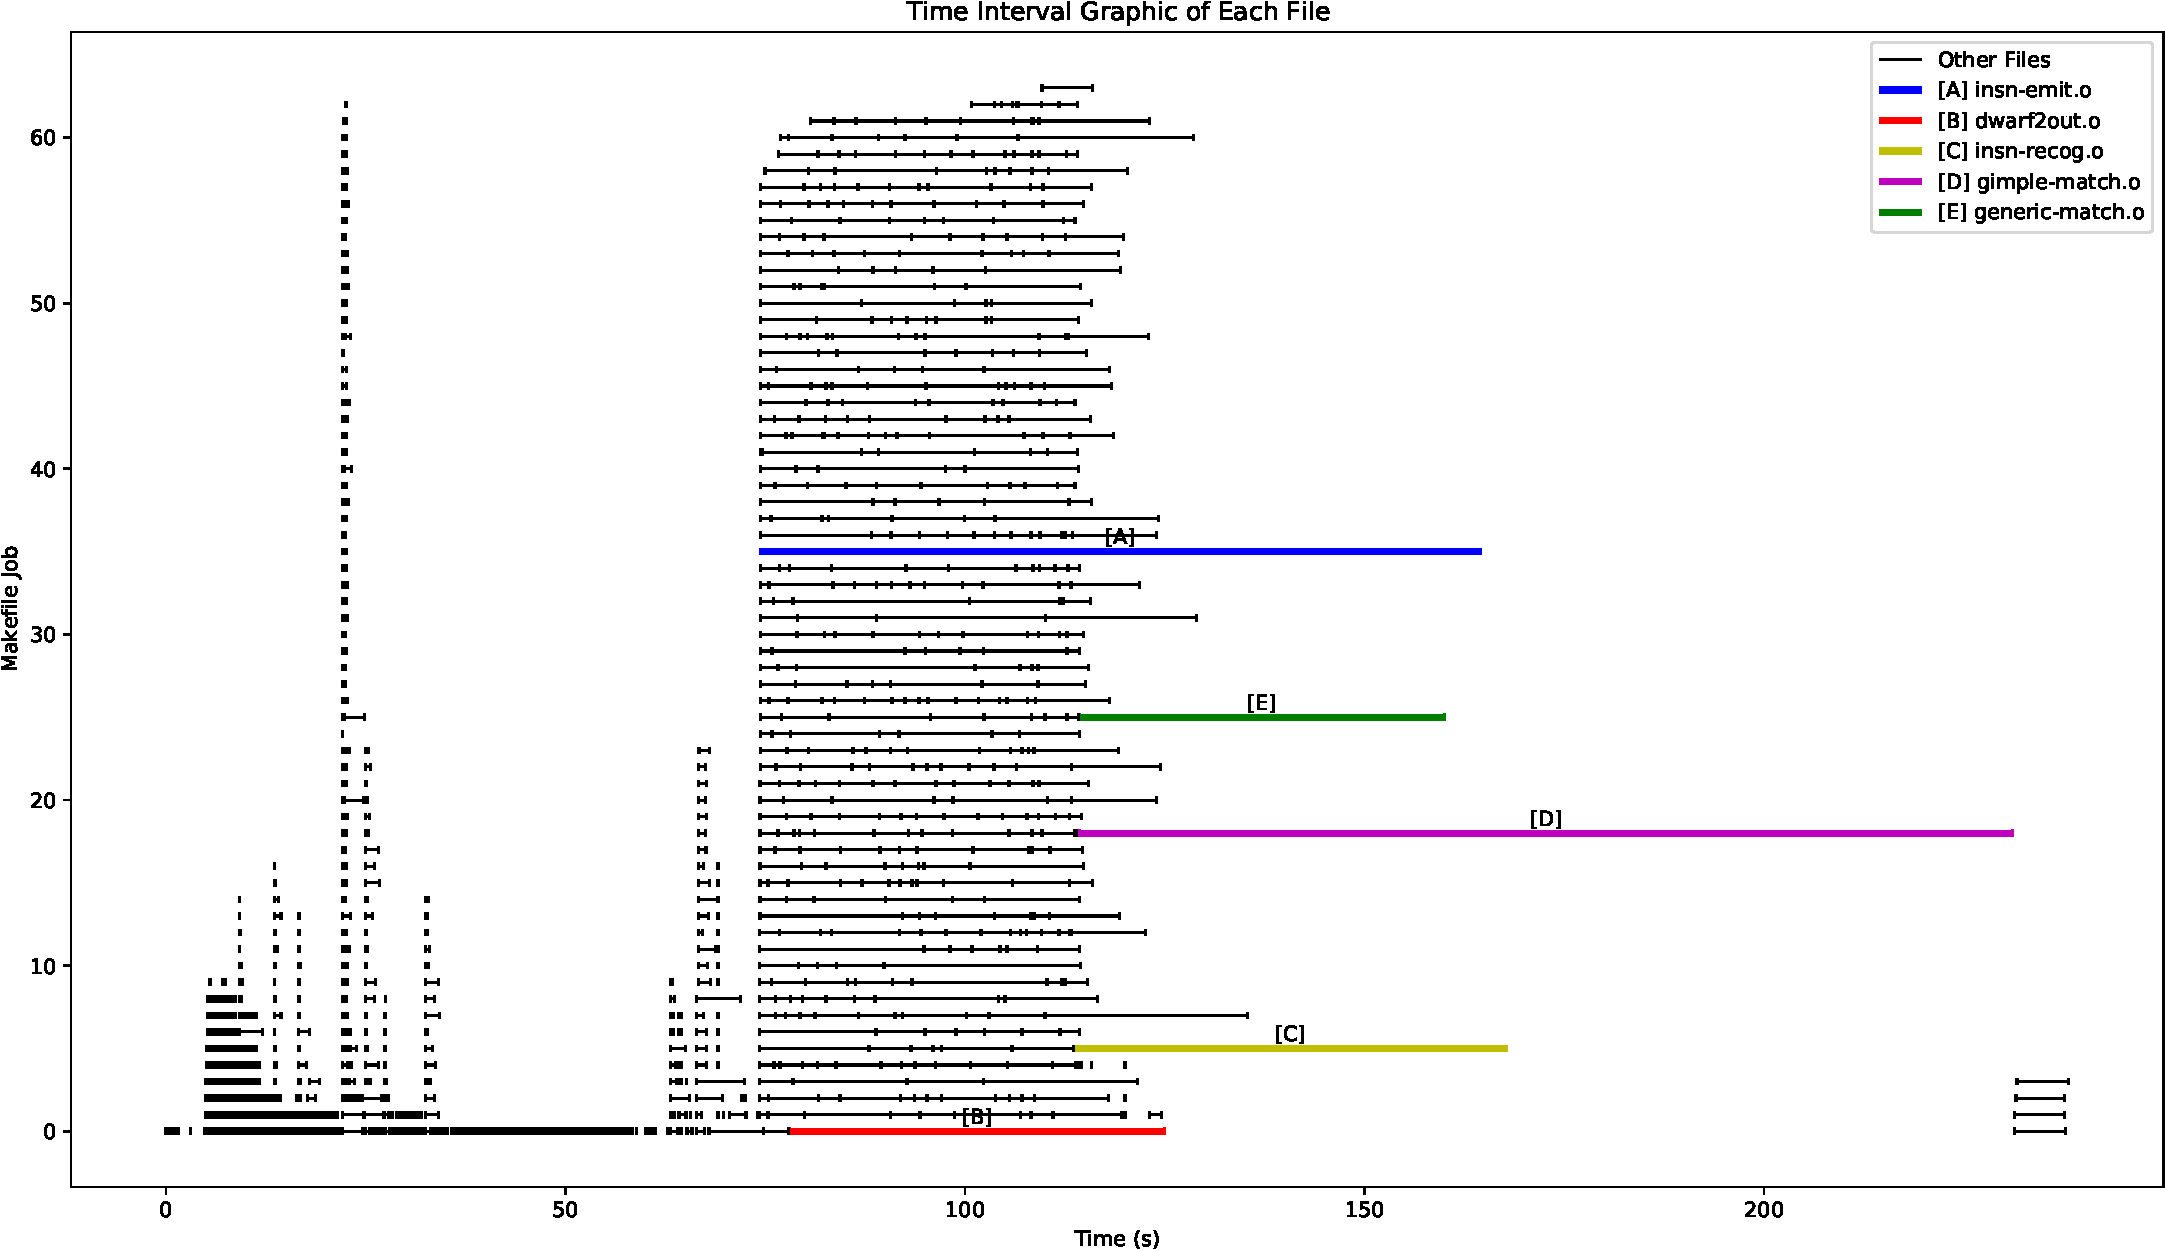
\includegraphics[width=0.9\paperheight]{seq-crop.pdf}
    \captionof{figure}{Compilation time of GCC without our modifications}
    \label{fig:analysis_classical}
%\end{figure}
\end{landscape}

\begin{landscape}
%\begin{figure}[ht]
 \vspace*{-2cm}%
 \noindent%
 \hspace*{-2cm}%
    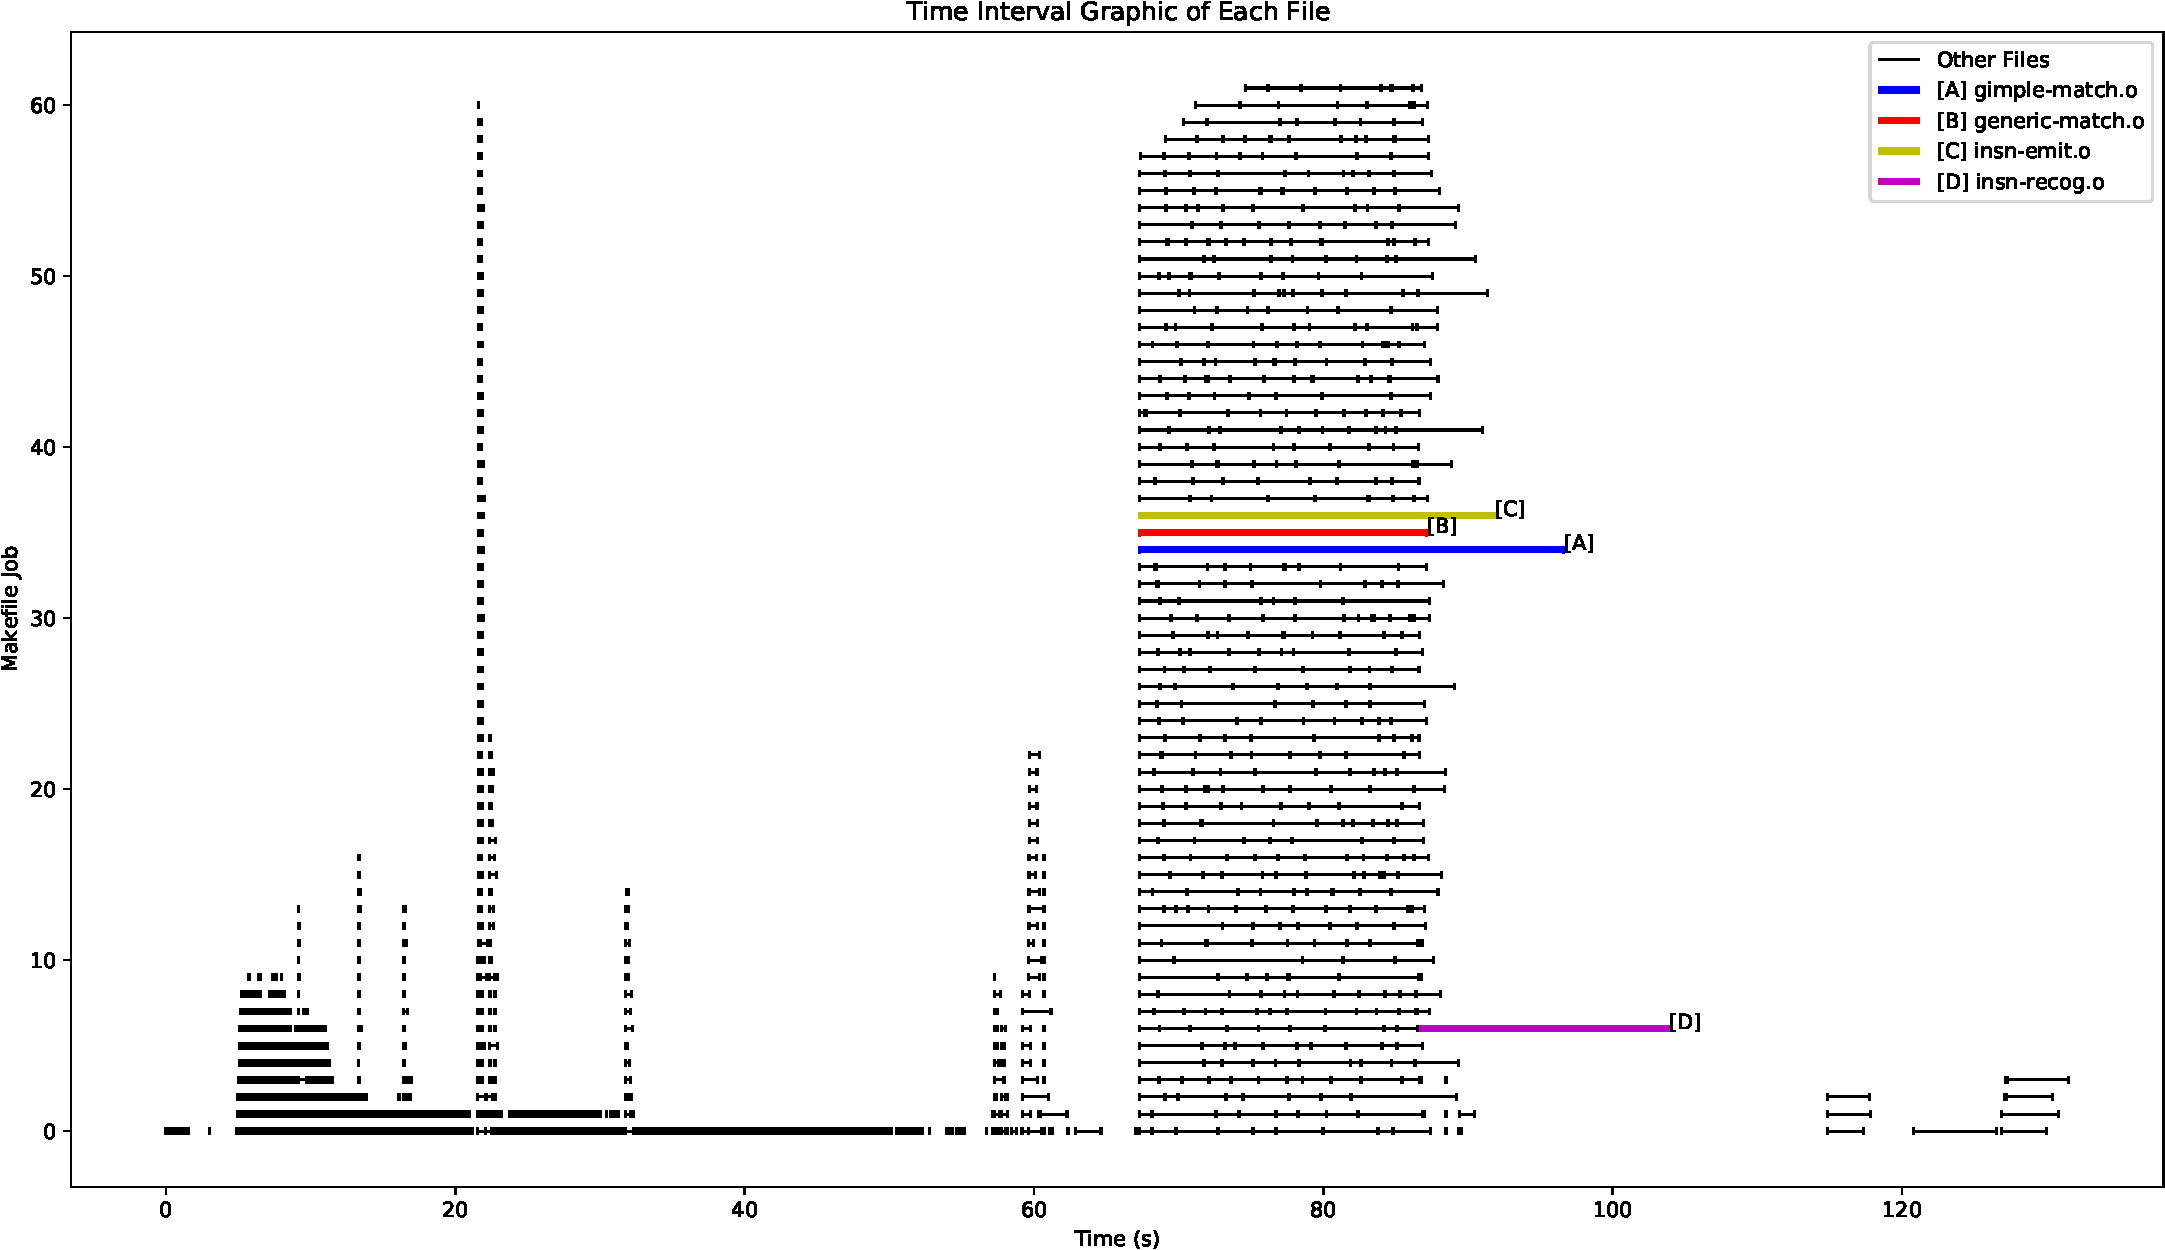
\includegraphics[width=0.9\paperheight]{par-crop.pdf}
    \captionof{figure}{Compilation time of GCC after our modifications}
    \label{fig:analysis_classical_parallel}
%\end{figure}
\end{landscape}

\begin{landscape}
%\begin{figure}[ht]
 \vspace*{-2cm}%
 \noindent%
 \hspace*{-2cm}%
    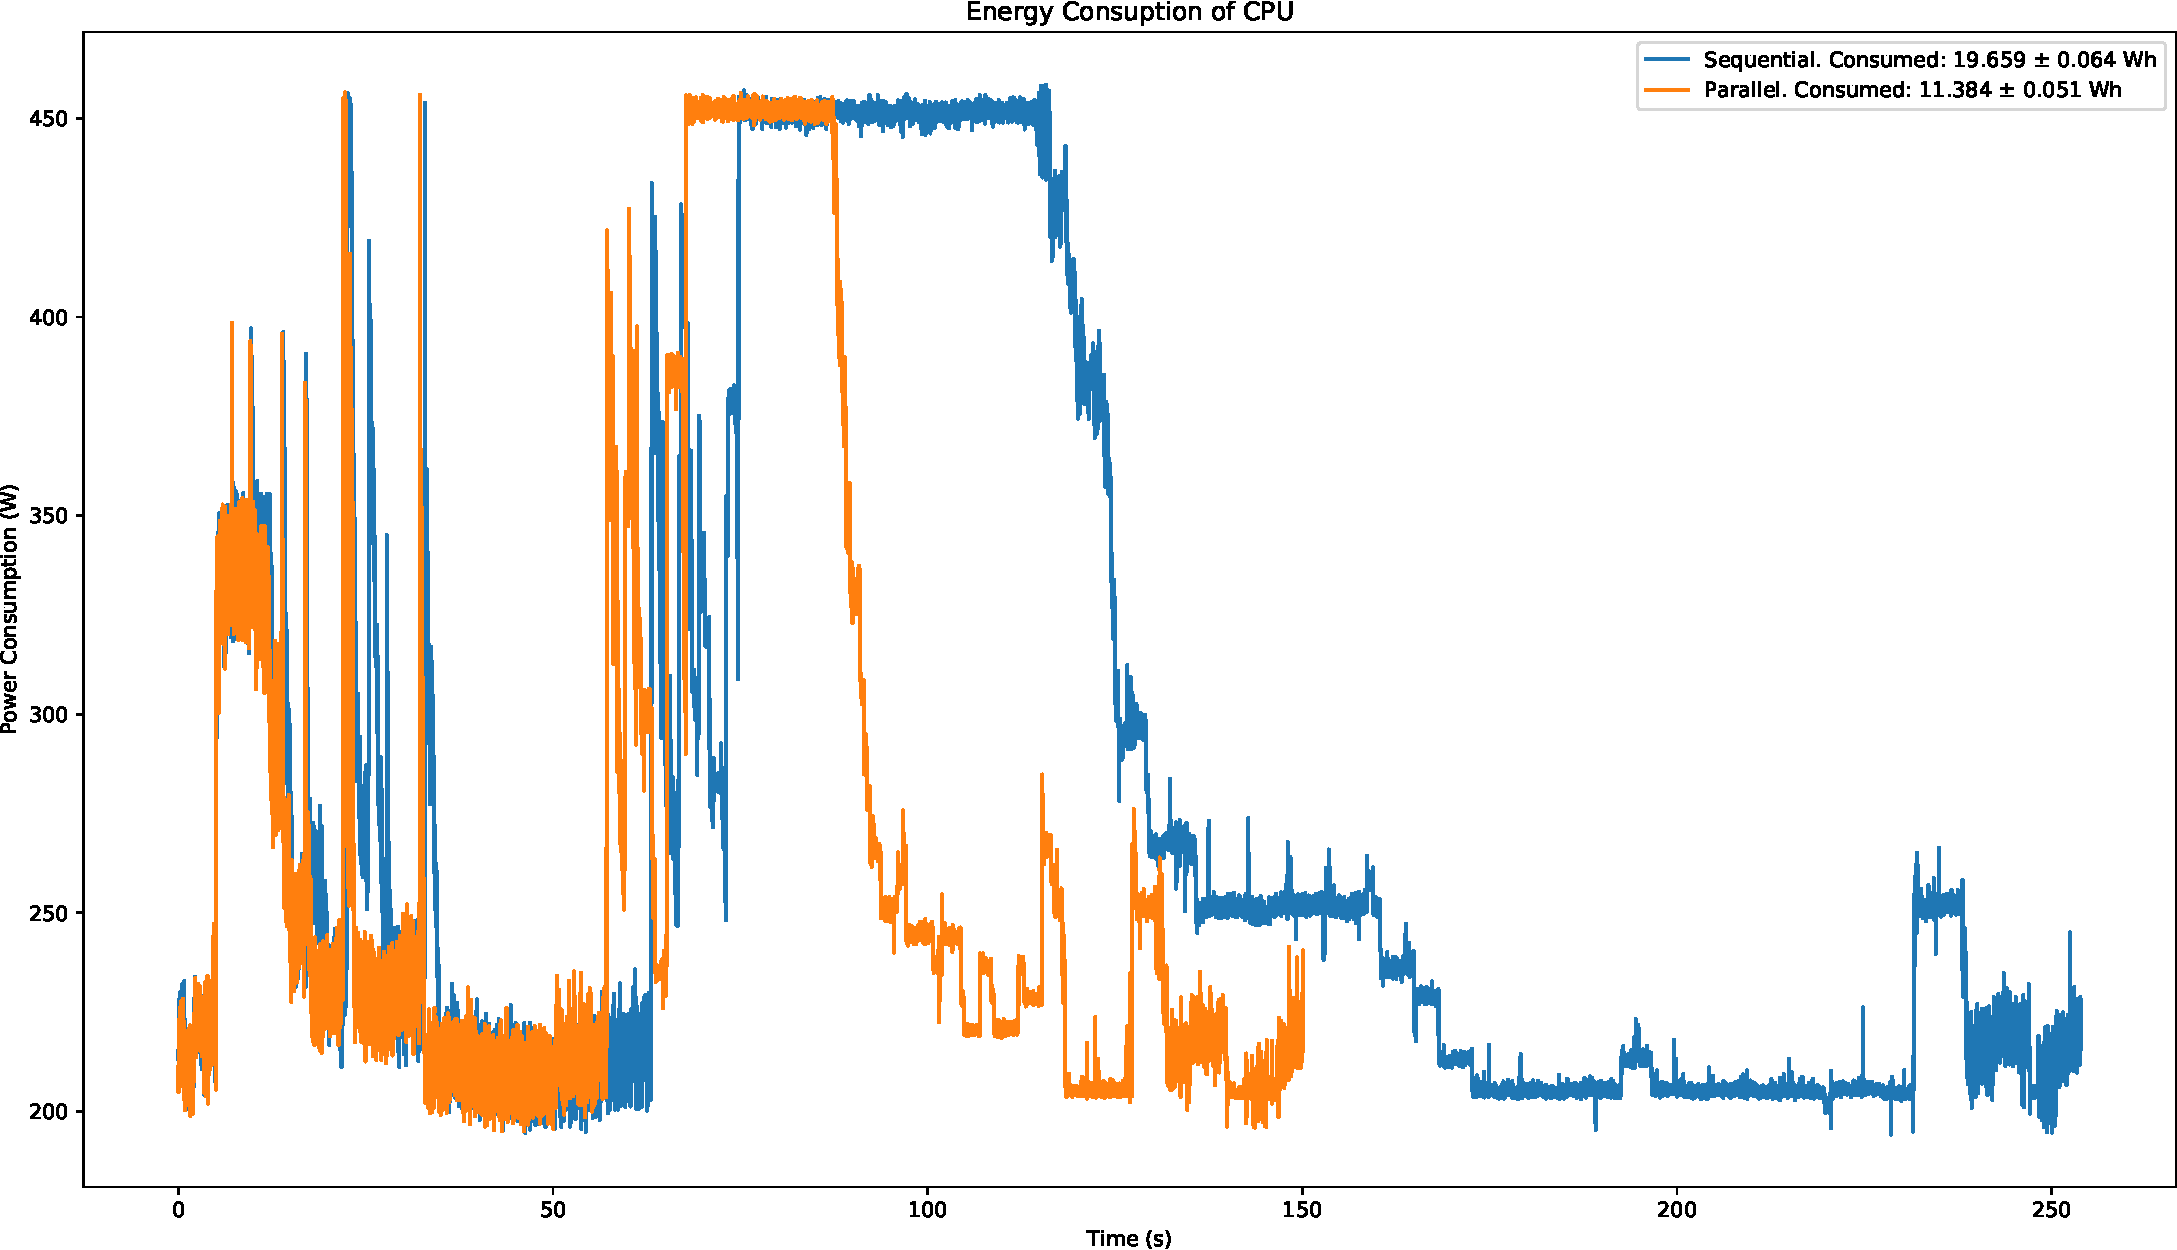
\includegraphics[width=0.9\paperheight]{power-crop.pdf}
    \captionof{figure}{Power usage comparison before and after our modifications}
    \label{fig:power}
%\end{figure}
\end{landscape}

\end{subsection}

\begin{subsection}{Feasibility Discussion}

We have presented a way to adapt the LTO engine to compile single files in
parallel. When compared to the threaded version, this work resulted in greater
speedups (2.4x vs. 1.61x) and less time required in development. This is
because lots of the LTO logic could be reused and the problem changed
drastically from ensuring that there are no race conditions to finding the
correct resources to share. Incremental development is also easier here, once
we knew that the sources of issues would be the partitioner or the partitioner
applier. Not only that, given an input file, the issues are reproducible,
removing the painful randomness of race conditions from the problem. 

The good news is that LTO is present in almost every industrial-scale compiler
nowadays. Therefore, implementing single-file parallelism on those by using our
methods would be significantly less cumbersome than making sure that the
threaded implementation is correct.

Therefore, if the compiler already has LTO support and the developers wants
to improve the performance of the compiler in manycore environments, this is a
quick to implement, large outcome method of doing that.


\end{subsection}

\begin{subsection}{Issues and Possible Improvements}
Our current LTO-based implementation can also be improved, which we highlight
some points of concern:
\begin{enumerate}

\item Fix the bugs which we already know. There is (1) a bug related
to how our partitioner applier handle nodes created by the \textit{ipa-split}
pass, and therefore we have disabled it for now; and (2) our partitioner
applier do not remove debug symbols associated with removed nodes, resulting in
unknown symbols being dumped into the final assembly. These bugs certainly prevents the
current branch from being used in industrial environments (which is a good
reason why this was not merged in upstream yet), but they are fine as a proof
of concept to support our claims.

\item Implementing a better partitioner to the project. One main issue
with our partitioner is that we kept its load balancing algorithm minimal to
ensure that it works. Using the LTO default partitioner as a base is a good start.

\item By modifying the driver to also support external compiler through GCC
SPEC language. Our current implementation only checks if launching program
is a known compiler/assembler/linker, and will get confused in languages that
needs additional steps (such as CUDA).

\item Try to develop a predictive model to decide if the input file is
a good candidate for parallel compilation. Fig. \ref{fig:gcc_all_files} shows
a clear linear correlation between the expected number of instructions and time
(and maybe it is the best parameter), but it may be possible to (statically)
collect more information about the file for a better decision.

\item Try to avoid partial linking and symbol promotion altogether by
concatenating the generated assembly files, instead of linking every generated
assembly file into temporary object files. This is extra useful for
architectures that require extra steps to generate code that must be globally
available across the program, which may generate a slower code when compared to
the non-public promoted version.

\end{enumerate}
\end{subsection}

\end{section}

%Neste capítulo é apresentado um plano de trabalho que será executado
%após o período de qualificação, bem como resultados esperados.
%Este trabalho tem o objetivo de trazer duas contribuições:
%\begin{enumerate}
%    \item Uma revisão sobre o que pode ser feito para acelerar o
%processo clássico de compilação em máquinas \textit{manycore} através
%de paralelismo, e quais problemas devem ser atacados em trabalhos futuros.
%
%    \item Uma opção no compilador GCC para que ele seja
%capaz de compilar um único arquivo em paralelo sem utilizar a
%estrutura do LTO. Isso é útil para desenvolvedores que trabalham
%com grandes softwares iterativamente, pois deve minimizar
%gargalos gerados por arquivos grandes e cobrir os casos onde o LTO gera
%binários menos eficientes, fornecendo assim uma alternativa a essa tecnologia.
%Este trabalho se concentra em paralelizar os passos de otimização Intra Procedural
%a nível de funções, ou seja, duas análises executarão em paralelo em funções
%distintas, evitando adentrar em paralelizar a análise de fluxo de dados. Espera-se
%utilizar as informações do item 1 para realizar um estudo de caso.
%\end{enumerate}
%O segundo item será enviado ao GCC como uma contribuição ao \textit{software}
%livre. O projeto de paralelização foi submetido e aprovado para o GSoC 2019,
%conforme o Apêndice \ref{ap:gsoc}.


%\section{Paralelização do GCC com \textit{threads}}
%
%Nesta subseção é apresentado o estado atual do projeto de paralelização
%do GCC com \textit{threads}. O GCC foi escolhido como candidato para
%paralelização pois a comunidade demonstrou grande interesse no projeto,
%conforme discutido na Seção \ref{cap:introducao}, e também devido a familiaridade
%do autor com o projeto, já tendo previamente contribuído com este. Sendo assim,
%utilizar outro compilador como o Clang para implementar o projeto demandaria
%estudos sobre a estrutura do projeto e convencimento da comunidade das possíveis
%vantagens deste trabalho ao projeto. Por outro lado, implementar um
%novo compilador não é uma alternativa viável dado que um dos maiores gargalos
%na compilação é o otimizador, peça que não seria possível implementar em
%dois anos com o mesmo poder das já existentes no GCC ou no Clang.
%
%Como atestado por \cite{PR84402}, há um gargalo de paralelismo dentro do
%próprio GCC por conta de arquivos grandes. Outro gargalo também foi relatado
%por \cite{mailgcc} em outro projeto interno. Uma das soluções para este
%problema é melhorar o paralelismo dentro do GCC, tornando possível fazer
%com que a compilação destes arquivos utilize mais núcleos de processamento.
%Nesta discussão, foi proposta uma maneira de visualizar o problema de
%paralelismo através de um gráfico gerado por dados de um GNU Make modificado.
%Como a alteração no Make é razoavelmente complicada e o \textit{script} proposto
%possuía sérios problemas de estabilidade, foi desenvolvida uma outra maneira
%de replicar os resultados.
%
%Como desenvolvido e publicado por \cite{gcctimer}, a ferramenta aqui proposta
%é capaz de coletar e exibir dados referente ao tempo de compilação
%de cada arquivo no GCC, incluindo os testes gerados pelo GNU Autotools.
%A ferramenta funciona da seguinte forma: há um programa escrito em C chamado
%\texttt{cc\_wrapper} que encapsula o compilador C e C++ do ambiente, no caso o 
%GCC e o G++. O caminho para estes compiladores são passados como um parâmetro
%da compilação do \texttt{cc\_wrapper} de maneira que os binários gerados os
%simulem. Em seguida o programa abre um novo processo através do \texttt{fork()},
%chamando o GCC/G++ com os parâmetros passados a ele sem alterações. O processo
%inicia a coleta do tempo, busca pelo nome do arquivo objeto a ser gerado, e
%aguarda o GCC chamado terminar. Essa busca foi codificada de maneira a ser
%muito eficiente, tento um pior caso $O(n)$ com uma constante muito baixa,
%onde $n$ é o número de parâmetros passados ao GCC. Em seguida, o programa
%escreve o tempo de início, tempo de fim, e o nome do arquivo em um arquivo
%de texto. Houve cautela para que não haja mistura de linhas
%no arquivo por razão de escrita simultânea no arquivo. Há também um \textit{script}
%em \textit{Bash} para reproduzir os resultados facilmente.
%
%Também é disponibilizado pelo autor um programa em \textit{Python} para análise dos
%resultados, responsável por gerar os gráficos conforme
%mostrado na Figura \ref{fig:analysis_classical}. Em um dos eixos há o
%tempo de execução, no outro há
%o trabalho do Makefile. Para construir o gráfico, é utilizado a técnica
%de coloração de grafos de intervalos: cada nó representa um intervalo de
%tempo, e é adicionado uma aresta entre esses nós caso haja intersecção nos
%intervalos. Em seguida, é executado um algoritmo guloso de coloração a
%partir do tempo de inicio. Como o grafo é de intervalos, esse algoritmo
%garante que a quantidade de cores utilizadas é a menor possível. Isso dá
%uma boa estimativa de como os trabalhos foram distribuidos pelo Makefile.
%Do ponto de vista de complexidade, isso garante que os gráficos podem ser
%gerados em $O(n \log p)$, onde $n$ é o número de arquivos e $p$ é o número de
%cores, embora o algoritmo implementado seja $O(np)$.
%
%\subsection{Investigação do Tempo Consumido na Compilação}
%
%Uma investigação foi conduzida com a finalidade de encontrar o gargalo
%principal no processo de compilação do GCC. Todos os testes efetuados foram
%executados em um computador com um AMD Opteron 6376 (64 núcleos) executando
%o Debian 10 (\textit{Testing}).
%
%Primeiro, foi executado um experimento com respeito ao tempo de compilação
%do GCC com o LTO habilitado, e outro desabilitado. Em ambos os experimentos,
%o processo de \textit{bootstrap} do compilador foi desabilitado. Para o caso LTO,
%utilizamos no máximo 64 \textit{threads} através da diretiva de compilação
%\texttt{-flto=64} para permitir o uso de paralelismo nesse método. Como
%é possível concluir comparando as Figuras \ref{fig:analysis_lto} e \ref{fig:analysis_classical},
%o LTO consome cerca de 1 minuto a mais para compilar todo o programa
%(mais de 200s do LTO, contra pouco mais de 140s sem o LTO). Sendo assim,
%desabilitar o LTO mesmo que ele forneça um grau maior de paralelismo é
%mais vantajoso caso o objetivo seja compilar mais rapidamente.
%
%Analisando o paralelismo do processo clássico na Figura \ref{fig:analysis_classical},
%é possível notar dois itens, independente da quantidade de
%execuções do experimento:
%
%\begin{itemize}
%    \item A existência de arquivos como o \texttt{gimple-match.c}, que
%        geram um gargalo no paralelismo do GCC.
%
%    \item Várias etapas sequênciais executadas pelo GNU Autoconf.
%\end{itemize}
%
%O arquivo \texttt{gimple-match.c} é gerado automaticamente compilando
%o arquivo \texttt{match.pd} para C. Na versão 9.0.1 do GCC, o arquivo
%gerado contém exatamente 99329 linhas de código. Espera-se que o tempo
%de compilação do \texttt{gimple-match.c} diminua, em conjunto com o tempo
%total de compilação, ao paralelizar o GCC com \textit{threads}.
%
%Analisando o tempo necessário para compilar o arquivo \texttt{gimple-match.c},
%foi possível notar que:
%\begin{itemize}
%    \item São necessários em média 76 segundos para compilar tal arquivo.
%
%    \item 91\% desse tempo (69 segundos) é utilizado na etapa de otimização
%        e geração de código final.
%
%    \item 8\% desse tempo (6 segundos) é utilizado na etapa de análise léxica
%        e sintática.
%
%    \item O outro 1\% está distribuído em diversas partes do compilador.
%\end{itemize}
%Todos estes dados foram obtidos autocompilando o GCC 9.0.1, e utilizando a
%ferramenta de \textit{profiling} incorporada
%no GCC através das flags \texttt{-ftime-report} \texttt{-ftime-report-details}.
%
%Como as otimizações do GCC são divididas em IPA, GIMPLE e RTL, é necessário
%executar uma granularidade mais fina na análise. Com uma simples alteração
%no GCC, foi possível separar a etapa IPA das demais. Bastou embrulhar as funções
%\texttt{ipa\_passes()} e \texttt{expand\_all\_functions()} com duas \textit{timevars}
%distintas. Assim, os seguintes dados foram obtidos:
%\begin{itemize}
%    \item 75\% do tempo total de compilação (57s) é gasto nos passos de otimização
%        Intra Procedural e geração de código.
%
%    \item 11\% do tempo total de compilação (11s) é gasto para realizar as IPA.
%\end{itemize}
%Sendo assim, o principal candidato a paralelização é a função \texttt{expand\_all\_functions()},
%responsável pelas otimizações Intra Procedural e geração de código.
%Entretanto, para realizar tal paralelização, será necessário documentar e remover diversas
%variáveis globais do GCC de maneira que seja possível realizar paralelismo com \textit{threads}.
%
%\subsection{Análise do \textit{Speedup} Máximo}
%
%Conforme analisado acima, se paralelizarmos as etapas de otimização Intra
%Procedural e Geração de Código, é possível paralelizar 75\% do tempo total.
%Portanto, seja $p$ o número de processadores utilizados. Assumindo
%\textit{speedup} linear, o ganho máximo será:
%
%$$ T_p = \frac{1}{4} T_1 + \frac{3}{4p}T_1 = \frac{1}{4} \left( 1 + \frac{3}{p}
%\right)T_1 $$ Sendo assim, o \textit{speedup} máximo por arquivo será: $$
%\lim_{p \rightarrow +\infty} \frac{T_1}{T_p} = \lim_{p \rightarrow +\infty}
%\frac{T_1}{\frac{1}{4} \left( 1 + \frac{3}{p} \right)T_1} = \lim_{p \rightarrow
%+\infty} \frac{4}{1 + \frac{3}{p}} = 4$$
%Entretanto, é muito provável que o \textit{speedup} a ser obtido seja menor que isto
%devido a mecanismos de sincronização necessários para implementar o paralelismo.
%
%\subsection{Arquitetura da Paralelização}
%
%A arquitetura da paralelização que será implementada no GCC é similar ao
%descrito por \cite{wortman1992}: serão executadas um número fixo de
%\textit{threads} trabalhadoras de acordo com o número de processadores
%disponíveis no computador.
%Assim que o IPA finalizar o plano de
%de otimização, as funções serão alimentadas em uma fila Produtor-Consumidor
%onde as \textit{threads} trabalhadoras retirarão o trabalho.
%Cada \textit{thread} será responsável por executar todas as passagens
%de otimização do GIMPLE em uma função retirada da fila produtor-consumidor.
%Sendo assim, duas \textit{threads} processarão duas funções distintas.
%Esse processo está retratado na Figura \ref{fig:paralelizacao}.
%Em seguida, será avaliado o \textit{speedup} ao paralelizar o GIMPLE, e
%será decidido qual outro problema abordar: paralelização das demais
%passagens RTL, ou uma tentativa de paralelizar o IPA.
%
%\begin{figure}[ht]
% \centering
% 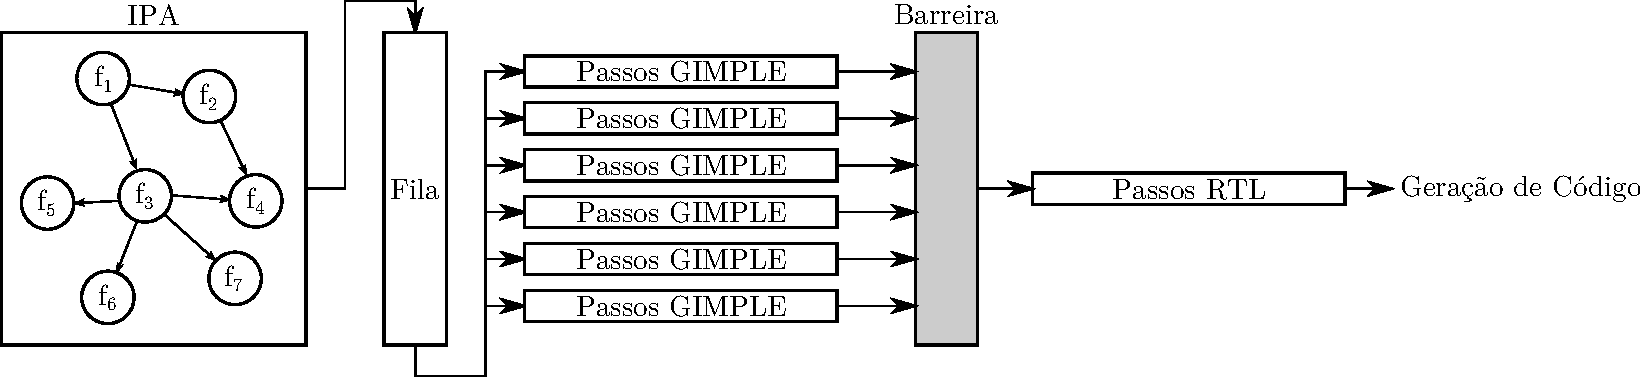
\includegraphics[width=\textwidth]{paralelizacao.pdf}
% \caption{Esquema de paralelização dos passos de otimização.}
% \label{fig:paralelizacao}
%\end{figure}
%\subsection{Experimentos e Metodologia}
%
%Para validar os resultados obtidos, serão executados dois experimentos:
%\begin{enumerate}
%    \item Comparação do tempo de compilação do arquivo \texttt{gimple-match.c}
%        antes e após a paralelização.
%
%
%    \item Comparação do tempo total de compilação do GCC antes e após a paralelização.
%\end{enumerate}
%Tal comparação será realizada utilizando
%técnicas de inferência estatística, conforme descrito por
%\cite{morettin2017estatistica}: serão
%coletadas diversas amostras a respeito do tempo de compilação. Em seguida, será feita alguma suposição a respeito da distribuição
%das amostras de acordo com o resultado de um gráfico Q-Q para então calcular um estimador
%para o valor esperado e variância. Com isso, serão calculados os intervalos de confiança
%sobre a média do tempo de execução para afirmar que ela diminui após a paralelização. Caso
%não seja possível encontrar uma distribuição adequada, será utilizado o Teorema do Limite
%Central com um número grande de amostras. Em seguida, esse resultado será comparado com o
%tempo de compilação utilizando a estrutura LTO, também utilizando as mesmas técnicas estatísticas.
%
%\subsection{Cronograma}
%
%As atividades serão dispostas pelos próximos meses na seguinte forma:
%
%\begin{figure}
%
%  \centering
%
%  \begin{ganttchart}{2019-05}{2020-3}
%    \gantttitlecalendar{year,month=shortname} \ganttnewline
%    \ganttgroup[progress=0]{Paralelização do GIMPLE}{2019-05}{2019-09} \ganttnewline
%    \ganttbar[progress=0]{Separar GIMPLE e RTL}{2019-05}{2019-05} \ganttnewline
%    \ganttbar[progress=0]{Remover estados Globais}{2019-05}{2019-07} \ganttnewline
%    \ganttbar[progress=0]{Paralelizar o GIMPLE}{2019-07}{2019-09} \ganttnewline
%    \ganttmilestone{Experimentos}{2019-09} \ganttnewline
%    \ganttgroup[progress=0]{Avaliar a paralelização do RTL e IPA}{2019-10}{2019-12} \ganttnewline
%    \ganttgroup[progress=0]{Escrita da Tese}{2019-11}{2020-02} \ganttnewline
%    \ganttbar[progress=0]{Escrita do Artigo}{2019-11}{2019-12} \ganttnewline
%    \ganttbar[progress=0]{Escrita do Tese}{2019-12}{2020-02} \ganttnewline
%    \ganttmilestone{Submissão}{2020-02}
%  \end{ganttchart}
%
%  \caption{Cronograma das Atividades.\label{fig:gantt}}
%\end{figure}
%
%\begin{itemize}
%	\item Separar GIMPLE e RTL: O RTL tem dependências com o \textit{Back End}
%	do GCC, sendo assim os passos GIMPLE e RTL serão separados para que seja
%	possível paralelizar os passos GIMPLE.
%
%	\item Remover estados globais: O GCC tem muitos estados globais referentes
%	aos passos GIMPLE que deverão ser adaptados para a paralelização.
%
%	\item Paralelizar o GIMPLE: Será adicionado código para que os passos do
%	GIMPLE executem em paralelo, e em seguida os experimentos serão executados.
%
%	\item Avaliar a paralelização do RTL e IPA: Dependendo do ganho obtido
%	na etapa anterior, será avaliado o ganho em paralelizar os passos IPA ou
%	o RTL.
%
%    \item Escrita de um Artigo Científico. Tempo destinado a escrita de um
%        artigo a respeito dos resultados do trabalho.
%
%	\item Escrita da Dissertação: Tempo destinado a escrita do texto final da
%        dissertação.
%\end{itemize}
%Uma ilustração da distribuição dessas tarefas no tempo está representada na
%Figura \ref{fig:gantt}.

%%%%%
